% Options for packages loaded elsewhere
\PassOptionsToPackage{unicode}{hyperref}
\PassOptionsToPackage{hyphens}{url}
%
\documentclass[
  ignorenonframetext,
]{beamer}
\usepackage{pgfpages}
\setbeamertemplate{caption}[numbered]
\setbeamertemplate{caption label separator}{: }
\setbeamercolor{caption name}{fg=normal text.fg}
\beamertemplatenavigationsymbolsempty
% Prevent slide breaks in the middle of a paragraph
\widowpenalties 1 10000
\raggedbottom
\setbeamertemplate{part page}{
  \centering
  \begin{beamercolorbox}[sep=16pt,center]{part title}
    \usebeamerfont{part title}\insertpart\par
  \end{beamercolorbox}
}
\setbeamertemplate{section page}{
  \centering
  \begin{beamercolorbox}[sep=12pt,center]{part title}
    \usebeamerfont{section title}\insertsection\par
  \end{beamercolorbox}
}
\setbeamertemplate{subsection page}{
  \centering
  \begin{beamercolorbox}[sep=8pt,center]{part title}
    \usebeamerfont{subsection title}\insertsubsection\par
  \end{beamercolorbox}
}
\AtBeginPart{
  \frame{\partpage}
}
\AtBeginSection{
  \ifbibliography
  \else
    \frame{\sectionpage}
  \fi
}
\AtBeginSubsection{
  \frame{\subsectionpage}
}
\usepackage{amsmath,amssymb}
\usepackage{lmodern}
\usepackage{iftex}
\ifPDFTeX
  \usepackage[T1]{fontenc}
  \usepackage[utf8]{inputenc}
  \usepackage{textcomp} % provide euro and other symbols
\else % if luatex or xetex
  \usepackage{unicode-math}
  \defaultfontfeatures{Scale=MatchLowercase}
  \defaultfontfeatures[\rmfamily]{Ligatures=TeX,Scale=1}
\fi
\usetheme[]{CambridgeUS}
% Use upquote if available, for straight quotes in verbatim environments
\IfFileExists{upquote.sty}{\usepackage{upquote}}{}
\IfFileExists{microtype.sty}{% use microtype if available
  \usepackage[]{microtype}
  \UseMicrotypeSet[protrusion]{basicmath} % disable protrusion for tt fonts
}{}
\makeatletter
\@ifundefined{KOMAClassName}{% if non-KOMA class
  \IfFileExists{parskip.sty}{%
    \usepackage{parskip}
  }{% else
    \setlength{\parindent}{0pt}
    \setlength{\parskip}{6pt plus 2pt minus 1pt}}
}{% if KOMA class
  \KOMAoptions{parskip=half}}
\makeatother
\usepackage{xcolor}
\newif\ifbibliography
\usepackage{color}
\usepackage{fancyvrb}
\newcommand{\VerbBar}{|}
\newcommand{\VERB}{\Verb[commandchars=\\\{\}]}
\DefineVerbatimEnvironment{Highlighting}{Verbatim}{commandchars=\\\{\}}
% Add ',fontsize=\small' for more characters per line
\usepackage{framed}
\definecolor{shadecolor}{RGB}{248,248,248}
\newenvironment{Shaded}{\begin{snugshade}}{\end{snugshade}}
\newcommand{\AlertTok}[1]{\textcolor[rgb]{0.94,0.16,0.16}{#1}}
\newcommand{\AnnotationTok}[1]{\textcolor[rgb]{0.56,0.35,0.01}{\textbf{\textit{#1}}}}
\newcommand{\AttributeTok}[1]{\textcolor[rgb]{0.77,0.63,0.00}{#1}}
\newcommand{\BaseNTok}[1]{\textcolor[rgb]{0.00,0.00,0.81}{#1}}
\newcommand{\BuiltInTok}[1]{#1}
\newcommand{\CharTok}[1]{\textcolor[rgb]{0.31,0.60,0.02}{#1}}
\newcommand{\CommentTok}[1]{\textcolor[rgb]{0.56,0.35,0.01}{\textit{#1}}}
\newcommand{\CommentVarTok}[1]{\textcolor[rgb]{0.56,0.35,0.01}{\textbf{\textit{#1}}}}
\newcommand{\ConstantTok}[1]{\textcolor[rgb]{0.00,0.00,0.00}{#1}}
\newcommand{\ControlFlowTok}[1]{\textcolor[rgb]{0.13,0.29,0.53}{\textbf{#1}}}
\newcommand{\DataTypeTok}[1]{\textcolor[rgb]{0.13,0.29,0.53}{#1}}
\newcommand{\DecValTok}[1]{\textcolor[rgb]{0.00,0.00,0.81}{#1}}
\newcommand{\DocumentationTok}[1]{\textcolor[rgb]{0.56,0.35,0.01}{\textbf{\textit{#1}}}}
\newcommand{\ErrorTok}[1]{\textcolor[rgb]{0.64,0.00,0.00}{\textbf{#1}}}
\newcommand{\ExtensionTok}[1]{#1}
\newcommand{\FloatTok}[1]{\textcolor[rgb]{0.00,0.00,0.81}{#1}}
\newcommand{\FunctionTok}[1]{\textcolor[rgb]{0.00,0.00,0.00}{#1}}
\newcommand{\ImportTok}[1]{#1}
\newcommand{\InformationTok}[1]{\textcolor[rgb]{0.56,0.35,0.01}{\textbf{\textit{#1}}}}
\newcommand{\KeywordTok}[1]{\textcolor[rgb]{0.13,0.29,0.53}{\textbf{#1}}}
\newcommand{\NormalTok}[1]{#1}
\newcommand{\OperatorTok}[1]{\textcolor[rgb]{0.81,0.36,0.00}{\textbf{#1}}}
\newcommand{\OtherTok}[1]{\textcolor[rgb]{0.56,0.35,0.01}{#1}}
\newcommand{\PreprocessorTok}[1]{\textcolor[rgb]{0.56,0.35,0.01}{\textit{#1}}}
\newcommand{\RegionMarkerTok}[1]{#1}
\newcommand{\SpecialCharTok}[1]{\textcolor[rgb]{0.00,0.00,0.00}{#1}}
\newcommand{\SpecialStringTok}[1]{\textcolor[rgb]{0.31,0.60,0.02}{#1}}
\newcommand{\StringTok}[1]{\textcolor[rgb]{0.31,0.60,0.02}{#1}}
\newcommand{\VariableTok}[1]{\textcolor[rgb]{0.00,0.00,0.00}{#1}}
\newcommand{\VerbatimStringTok}[1]{\textcolor[rgb]{0.31,0.60,0.02}{#1}}
\newcommand{\WarningTok}[1]{\textcolor[rgb]{0.56,0.35,0.01}{\textbf{\textit{#1}}}}
\usepackage{longtable,booktabs,array}
\usepackage{calc} % for calculating minipage widths
\usepackage{caption}
% Make caption package work with longtable
\makeatletter
\def\fnum@table{\tablename~\thetable}
\makeatother
\setlength{\emergencystretch}{3em} % prevent overfull lines
\providecommand{\tightlist}{%
  \setlength{\itemsep}{0pt}\setlength{\parskip}{0pt}}
\setcounter{secnumdepth}{-\maxdimen} % remove section numbering
\usepackage{amsmath}
\ifLuaTeX
  \usepackage{selnolig}  % disable illegal ligatures
\fi
\IfFileExists{bookmark.sty}{\usepackage{bookmark}}{\usepackage{hyperref}}
\IfFileExists{xurl.sty}{\usepackage{xurl}}{} % add URL line breaks if available
\urlstyle{same} % disable monospaced font for URLs
\hypersetup{
  pdftitle={Efficient Management of Data in R (Data Structures!)},
  hidelinks,
  pdfcreator={LaTeX via pandoc}}

\title{Efficient Management of Data in R (Data Structures!)}
\subtitle{Data Science Lecture Series: Advanced R}
\author{W. Evan Johnson, Ph.D.\\
Professor, Division of Infectious Disease\\
Director, Center for Data Science\\
Rutgers University -- New Jersey Medical School}
\date{2023-03-27}

\begin{document}
\frame{\titlepage}

\hypertarget{importing-data}{%
\section{Importing data}\label{importing-data}}

\begin{frame}[fragile]{Importing data}
\protect\hypertarget{importing-data-1}{}
The first problem a data scientist will usually face is how to import
data into R! \vskip .2in

Often they have to import data from either a file, a database, or other
sources. One of the most common ways of storing and sharing data for
analysis is through electronic spreadsheets. \vskip .2in

A spreadsheet stores data in rows and columns. It is basically a file
version of a * \texttt{data\ frame} (or a \texttt{tibble!}).
\end{frame}

\begin{frame}[fragile]{Importing data}
\protect\hypertarget{importing-data-2}{}
A common function for importing data is the \texttt{read.table}
function:

\begin{Shaded}
\begin{Highlighting}[]
\NormalTok{mydata }\OtherTok{\textless{}{-}} \FunctionTok{read.table}\NormalTok{(}\StringTok{"mydata.txt"}\NormalTok{)}
\end{Highlighting}
\end{Shaded}

This is looking for a structured dataset, with the same number of
entries in each row, and data that is delimited with a single space
between values.
\end{frame}

\begin{frame}[fragile]{Importing data}
\protect\hypertarget{importing-data-3}{}
The \texttt{read.table} function can also read tab-delimited data:

\begin{Shaded}
\begin{Highlighting}[]
\NormalTok{mydata }\OtherTok{\textless{}{-}} \FunctionTok{read.table}\NormalTok{(}\StringTok{"mydata.txt"}\NormalTok{, }\AttributeTok{sep=}\StringTok{"}\SpecialCharTok{\textbackslash{}t}\StringTok{"}\NormalTok{)}
\end{Highlighting}
\end{Shaded}

\vskip .2in Or comma separated (.csv) formats:

\begin{Shaded}
\begin{Highlighting}[]
\NormalTok{mydata }\OtherTok{\textless{}{-}} \FunctionTok{read.table}\NormalTok{(}\StringTok{"mydata.txt"}\NormalTok{, }\AttributeTok{sep=}\StringTok{","}\NormalTok{)}
\end{Highlighting}
\end{Shaded}

(also explore the \{\bf read.csv\} function)
\end{frame}

\begin{frame}[fragile]{Importing data}
\protect\hypertarget{importing-data-4}{}
We can also add options to set the first column as a header and select a
row for the row labels:

\begin{Shaded}
\begin{Highlighting}[]
\NormalTok{mydata }\OtherTok{\textless{}{-}} \FunctionTok{read.table}\NormalTok{(}\StringTok{"mydata.txt"}\NormalTok{,}
                     \AttributeTok{header=}\ConstantTok{TRUE}\NormalTok{,}
                     \AttributeTok{row.names=}\StringTok{"id"}\NormalTok{)}
\end{Highlighting}
\end{Shaded}
\end{frame}

\begin{frame}[fragile]{Importing data}
\protect\hypertarget{importing-data-5}{}
Excel files can also be directly imported using \texttt{read.xlsx}:

\begin{Shaded}
\begin{Highlighting}[]
\FunctionTok{library}\NormalTok{(xlsx)}
\NormalTok{mydata }\OtherTok{\textless{}{-}} \FunctionTok{read.xlsx}\NormalTok{(}\StringTok{"myexcel.xlsx"}\NormalTok{)}
\end{Highlighting}
\end{Shaded}

\vskip .2in And one can also select a specific sheet in the Excel file:

\begin{Shaded}
\begin{Highlighting}[]
\NormalTok{mydata }\OtherTok{\textless{}{-}} \FunctionTok{read.xlsx}\NormalTok{(}\StringTok{"myexcel.xlsx"}\NormalTok{, }
                    \AttributeTok{sheetName =} \StringTok{"mysheet"}\NormalTok{)}
\end{Highlighting}
\end{Shaded}
\end{frame}

\begin{frame}[fragile]{Other functions for importing data}
\protect\hypertarget{other-functions-for-importing-data}{}
Other useful importing tools are \texttt{scan}, \texttt{readLines},
\texttt{readr}, and \texttt{readxl}. The latter two we will discuss
later.
\end{frame}

\hypertarget{introduction-to-data-structures}{%
\section{Introduction to Data
Structures}\label{introduction-to-data-structures}}

\begin{frame}{Importance of data structures}
\protect\hypertarget{importance-of-data-structures}{}
A data structure is a particular way of organizing data in a computer so
that it can be used effectively. The idea is to reduce the space and
time complexities of different tasks. \vskip .2in

Data structures in R programming are tools for holding multiple values,
variables, and sometimes functions.\vskip .2in

Please think very carefully about the way you manage and store your
data! This can make your life much easier and make your code and data
cleaner and more portable!
\end{frame}

\begin{frame}{Types of data structures in R}
\protect\hypertarget{types-of-data-structures-in-r}{}
R's base data structures are often organized by their dimensionality
(1D, 2D, nD) and whether they're homogeneous or heterogeneous (elements
of identical or various type). Six of the most common data types are:

\begin{enumerate}
\tightlist
\item
  Vectors
\item
  Lists
\item
  Matrices
\item
  Arrays
\item
  Factors
\item
  Data frames (or tibbles)
\end{enumerate}
\end{frame}

\hypertarget{data-frames}{%
\section{Data Frames}\label{data-frames}}

\begin{frame}{Data Frames}
\protect\hypertarget{data-frames-1}{}
The most common data structure for storing a dataset in R is in a
\textbf{data frame}. Conceptually, we can think of a data frame as a two
dimensional table with rows representing observations and the different
variables reported for each observation defining the columns. Data
frames are particularly useful for datasets because we can combine
different data types into one object.
\end{frame}

\begin{frame}[fragile]{Data Frames}
\protect\hypertarget{data-frames-2}{}
We can convert matrices into data frames using the function
\texttt{as.data.frame}:

\begin{Shaded}
\begin{Highlighting}[]
\NormalTok{mat }\OtherTok{\textless{}{-}} \FunctionTok{matrix}\NormalTok{(}\DecValTok{1}\SpecialCharTok{:}\DecValTok{12}\NormalTok{, }\DecValTok{4}\NormalTok{, }\DecValTok{3}\NormalTok{)}
\NormalTok{mat }\OtherTok{\textless{}{-}} \FunctionTok{as.data.frame}\NormalTok{(mat)}
\end{Highlighting}
\end{Shaded}

\vskip .1in

Or just generate it directly using the \texttt{data.frame} function:

\begin{Shaded}
\begin{Highlighting}[]
\NormalTok{dat }\OtherTok{\textless{}{-}} \FunctionTok{data.frame}\NormalTok{(}\AttributeTok{x=}\DecValTok{1}\SpecialCharTok{:}\DecValTok{4}\NormalTok{, }\AttributeTok{y=}\DecValTok{5}\SpecialCharTok{:}\DecValTok{8}\NormalTok{, }\AttributeTok{z=}\DecValTok{9}\SpecialCharTok{:}\DecValTok{12}\NormalTok{)}
\end{Highlighting}
\end{Shaded}

\vskip .1in

A \texttt{data.frame} can be indexed as matrices,
\texttt{dat{[}1:2,\ 2:3{]}}, and columns can be extracted using the
\texttt{\$} operator.
\end{frame}

\hypertarget{tibbles}{%
\section{Tibbles}\label{tibbles}}

\begin{frame}[fragile]{Tibbles}
\protect\hypertarget{tibbles-1}{}
Here is a printed version of the data frame:

\begin{Shaded}
\begin{Highlighting}[]
\NormalTok{dat}
\end{Highlighting}
\end{Shaded}

\begin{verbatim}
##   x y  z
## 1 1 5  9
## 2 2 6 10
## 3 3 7 11
## 4 4 8 12
\end{verbatim}
\end{frame}

\begin{frame}[fragile]{Tibbles\}}
\protect\hypertarget{tibbles-2}{}
A \textbf{tibble} is a modern version of a data.frame.

\begin{Shaded}
\begin{Highlighting}[]
\FunctionTok{library}\NormalTok{(tidyverse)}
\NormalTok{dat1 }\OtherTok{\textless{}{-}} \FunctionTok{tibble}\NormalTok{(}\AttributeTok{x=}\DecValTok{1}\SpecialCharTok{:}\DecValTok{4}\NormalTok{, }\AttributeTok{y=}\DecValTok{5}\SpecialCharTok{:}\DecValTok{8}\NormalTok{, }\AttributeTok{z=}\DecValTok{9}\SpecialCharTok{:}\DecValTok{12}\NormalTok{)}
\end{Highlighting}
\end{Shaded}

\vskip .1in

Or convert a data.frame to a tibble

\begin{Shaded}
\begin{Highlighting}[]
\NormalTok{dat }\OtherTok{\textless{}{-}} \FunctionTok{data.frame}\NormalTok{(}\AttributeTok{x=}\DecValTok{1}\SpecialCharTok{:}\DecValTok{4}\NormalTok{, }\AttributeTok{y=}\DecValTok{5}\SpecialCharTok{:}\DecValTok{8}\NormalTok{, }\AttributeTok{z=}\DecValTok{9}\SpecialCharTok{:}\DecValTok{12}\NormalTok{)}
\NormalTok{dat1 }\OtherTok{\textless{}{-}} \FunctionTok{as\_tibble}\NormalTok{(dat)}
\end{Highlighting}
\end{Shaded}

\vskip .1in
\end{frame}

\begin{frame}[fragile]{Tibbles}
\protect\hypertarget{tibbles-3}{}
Here is a printed version of the tibble:

\begin{Shaded}
\begin{Highlighting}[]
\NormalTok{dat1}
\end{Highlighting}
\end{Shaded}

\begin{verbatim}
## # A tibble: 4 x 3
##       x     y     z
##   <int> <int> <int>
## 1     1     5     9
## 2     2     6    10
## 3     3     7    11
## 4     4     8    12
\end{verbatim}
\end{frame}

\begin{frame}[fragile]{Tibbles}
\protect\hypertarget{tibbles-4}{}
Important characteristics that make tibbles unique:

\begin{enumerate}
\tightlist
\item
  Tibbles are primary data structure for the \texttt{tidyverse}
\item
  Tibbles display better and printing is more readable
\item
  Tibbles can be grouped
\item
  Subsets of tibbles are tibbles
\item
  Tibbles can have complex entries--numbers, strings, logicals, lists,
  functions.
\item
  Tibbles can (almost) enable object-orientated programming in R
\end{enumerate}
\end{frame}

\hypertarget{advanced-data-structures-in-r}{%
\section{Advanced Data Structures in
R}\label{advanced-data-structures-in-r}}

\begin{frame}{Advanced Data Structures in R}
\protect\hypertarget{advanced-data-structures-in-r-1}{}
In your homework, you will explore more advanced R data structures,
namely the \textbf{S3} and \textbf{S4} class objects. These can
facilitate object orientated programming. \vskip .1in
\end{frame}

\begin{frame}{Advanced Data Structures in R}
\protect\hypertarget{advanced-data-structures-in-r-2}{}
One example of an S4 class data structure is the
\textbf{SummarizedExperiment} object.

\begin{center}
    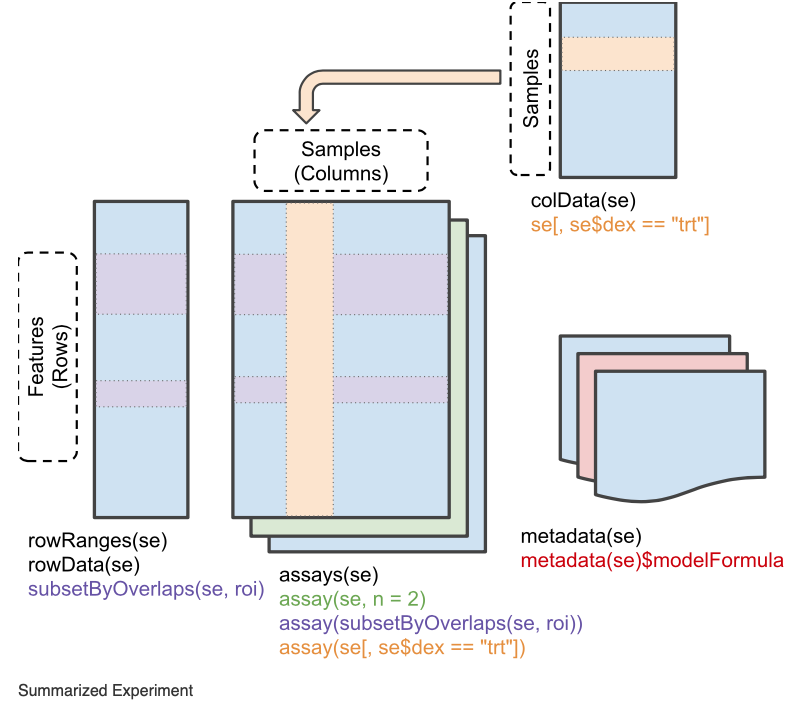
\includegraphics[width=2.75in]{figs/SummarizedExperiment.png}   
\end{center}
\end{frame}

\begin{frame}[fragile]{Session info}
\protect\hypertarget{session-info}{}
\tiny

\begin{Shaded}
\begin{Highlighting}[]
\FunctionTok{sessionInfo}\NormalTok{()}
\end{Highlighting}
\end{Shaded}

\begin{verbatim}
## R version 4.2.3 (2023-03-15)
## Platform: aarch64-apple-darwin20 (64-bit)
## Running under: macOS Ventura 13.3.1
## 
## Matrix products: default
## BLAS:   /Library/Frameworks/R.framework/Versions/4.2-arm64/Resources/lib/libRblas.0.dylib
## LAPACK: /Library/Frameworks/R.framework/Versions/4.2-arm64/Resources/lib/libRlapack.dylib
## 
## locale:
## [1] en_US.UTF-8/en_US.UTF-8/en_US.UTF-8/C/en_US.UTF-8/en_US.UTF-8
## 
## attached base packages:
## [1] stats     graphics  grDevices utils     datasets  methods   base     
## 
## other attached packages:
##  [1] lubridate_1.9.2 forcats_1.0.0   stringr_1.5.0   dplyr_1.1.1    
##  [5] purrr_1.0.1     readr_2.1.4     tidyr_1.3.0     tibble_3.2.1   
##  [9] ggplot2_3.4.2   tidyverse_2.0.0
## 
## loaded via a namespace (and not attached):
##  [1] pillar_1.9.0     compiler_4.2.3   tools_4.2.3      digest_0.6.31   
##  [5] timechange_0.2.0 evaluate_0.20    lifecycle_1.0.3  gtable_0.3.3    
##  [9] pkgconfig_2.0.3  rlang_1.1.0      cli_3.6.1        rstudioapi_0.14 
## [13] yaml_2.3.7       xfun_0.38        fastmap_1.1.1    withr_2.5.0     
## [17] knitr_1.42       generics_0.1.3   vctrs_0.6.1      hms_1.1.3       
## [21] grid_4.2.3       tidyselect_1.2.0 glue_1.6.2       R6_2.5.1        
## [25] fansi_1.0.4      rmarkdown_2.21   tzdb_0.3.0       magrittr_2.0.3  
## [29] scales_1.2.1     htmltools_0.5.5  colorspace_2.1-0 utf8_1.2.3      
## [33] stringi_1.7.12   munsell_0.5.0
\end{verbatim}
\end{frame}

\end{document}
